As we saw in the previous section, a suitable quasi-linear system enables the computation of the complete solution of a Riemann problems in solid dynamics. However, such a procedure may become complicated due to the non-linearity of the Jacobian matrix. Indeed, some problems can lead to the inability to derive explicit conditions as those developed for the Saint-Venant-Kirchhoff material \eqref{eq:1S2R_solution} and \eqref{eq:1R2S_solution}.

Numerical methods such as Finite Volume Methods \cite{Leveque} require the solution of many Riemann problems within a discretized medium. When dealing with non-linear problems, the exact solution of those problems may increase drastically the computational cost, making the numerical scheme prohibitive. Moreover numerical procedures often require little information about the solution of Riemann problems only and do not need the complete resolution. In that context, alternative procedures have been developed in order to take into account the characteristic structure of a hyperbolic system by computing an approximate solution of the Riemann problems. Approximate Riemann solvers developed for Computational Fluid Dynamics allow to extract information for either flux functions (\textit{HLL, HLLC, Roe} and \textit{Osher} approximate Riemann solvers \cite{Trangenstein}, \cite{Toro}) or approximate conserved quantities vectors. Some of those have been applied to specific solid mechanics problems such as the Osher \cite{LEE_FVM}, \cite{Haider_FVM} or the HLLC \cite{Ortega_HLLD} approximate solvers for hyperelasticity .

We recall here the formulation of the approximate-state Riemann solver \cite[Chapter~9]{Toro}, applied to solid mechanics \cite[Chapter~22]{Leveque}. Two examples are considered as illustrations
\begin{itemize}
\item[(i)] a hyperelastic Saint-Venant-Kirchhoff medium so that the comparison with the analytical solution developed in section \ref{subsec:charac_nonlinear_problems} can be made
\item[(ii)] an elastoplastic bar which constitutive model involves a particular procedure in the Riemann solver in order to manage the jump of characteristic speeds due to the crossing of the plastic threshold.\todo{citation ?}
\end{itemize}


\subsection{General ideas}
As in previous the section, we consider a Riemann solver in a direction $\vect{N}$ of the space:
\begin{equation}
  \label{eq:RP_approx}
  \begin{aligned}
  &\Qcb_t + \Jbsf\(\Qcb\) \drond{\Qcb}{X_N} = \vect{0}, \\
  &\left\lbrace 
    \begin{aligned}
      & \Qcb(X_N,t=0) = \Qcb^L \quad \text{if } X_N< 0\\
      & \Qcb(X_N,t=0) = \Qcb^R \quad \text{if } X_N> 0
    \end{aligned}
    \right.
  \end{aligned}
\end{equation}
The classical approach for developping an approximate-state Riemann solver is to first linearized the problem \eqref{eq:RP_approx} by assuming that $\Jbsf\approx \Jbsf\(\Qcb^L,\Qcb^R\)$ in the vicinity of $\Qcb^L$ and $\Qcb^R$ \cite[Chapter~15]{Leveque}. The constant matrix thus obtained $\bar{\Jbsf}=\Jbsf\(\Qcb^L,\Qcb^R\)$ must however ensure the hyperbolicity of the system ($\bar{\Jbsf}$ has real eigenvalues and a complete set of independent eigenvectors) and satisfy the consistency condition:
\begin{equation}
  \label{eq:approx_constistency}
  \bar{\Jbsf}\(\Qcb,\Qcb\)=\Jbsf\(\Qcb\)
\end{equation}
The eigenvalues $c_p$ and right eigenvectors $\Rcb^p$ of the Jacobian matrix are defined so that $\Jbsf \Rbsf = \Rbsf \Cbsf$ where $\Rbsf_{ij}=\Rcb^j_i$ is the (non-singular) matrix of right eigenvectors. In the general case, the characteristic speeds depend on $\Qcb$ so that one can assume that left-going (\textit{resp. right-going}) characteristics depend on $\Qcb^L$ (\textit{resp. on} $\Qcb^R$) only. In addition, the corresponding eigenvectors are also taken as function of $\Qcb$ on each side of the initial discontinuity. With matrices $\Rbsf$ defined as mentioned previously, the constant Jacobian matrix is $\Jbsf = \Rbsf \Cbsf \Rbsf^{-1}$ which obviously satisfy the consistency condition \eqref{eq:approx_constistency}.

At last, every state vector $\Qcb(x,t)$ can be determined by following the procedure described in section \ref{subsec:charac_Linear_problems}, namely by solving either equation \eqref{eq:jump_star_R} or \eqref{eq:jump_star_L}.


\begin{remark}
  The linearization approach developed above amounts to considering a heterogeneous medium where $\Qcb^{L}$ and $\Qcb^R$ act as material parameters.
\end{remark}

\subsection{Saint-Venant-Kirchhoff material}
We consider again the non-linear problem of section \ref{subsec:charac_nonlinear_problems} in order to see the influence of the approximation and the amount of information lost. Recall that for a one-dimensional problem in a solid made of a Saint-Venant-Kirchhoff material, the eigenvalues and right eigenvectors matrices reads:
\begin{equation}
  \label{eq:SVK_matrices}
  \Cbsf = \matrice{-c & 0 \\ 0 & c} \quad ; \quad \Rbsf = \matrice{c & -c\\ 1&1} \:,\quad c=\sqrt{\frac{\lambda + 2\mu}{2\rho_0}(3F^2-1)}
\end{equation}
Hence, the linearized problem is written with:
\begin{equation}
  \label{eq:SVK_matrices_linear}
  \Cbsf = \matrice{-c_L & 0 \\ 0 & c_R} \quad ; \quad \Rbsf = \matrice{c_L & -c_R\\ 1&1}
\end{equation}
In section \ref{subsec:charac_Linear_problems}, the expression of the wave strength vector $\vect{\delta}$ has been established for general linear systems of dimension $2$ (equation \eqref{eq:wave_strengths}). For the problem considered here we have:
\begin{equation}
  \vect{\delta}=\frac{1}{c_R+c_L}\matrice{c_R \Delta F +\Delta v\\ c_L \Delta F -\Delta v}
\end{equation}
leading to the solution between $\Qcb^*$ the two discontinuous waves:
\begin{equation}
  \label{eq:SVK_approx_solution}
  \Qcb^* = \Qcb^L + \delta^1 \Rcb^1 = \matrice{v_L \\F_L} +\delta^1 \matrice{c_L \\1} \quad \text{or} \quad \Qcb^* = \Qcb^R - \delta^2 \Rcb^2 = \matrice{v_R \\F_R} -\delta^2 \matrice{-c_R \\1}
\end{equation}
Substitutions of $\delta^{1,2}$ from second equations in first ones provide straight lines equations in the phase plane ($F,v$):
\begin{equation}
  \label{eq:approx_straight}
  v_* = v_L + c_L(F_*-F_L) \quad ; \quad v_* = v_R + c_R(F_R-F_*)
\end{equation}

\begin{figure}[h!]
  \centering
  {\definecolor{Purple}{RGB}{120,28,129}
\definecolor{Blue}{RGB}{63,96,174}
\definecolor{Duck}{RGB}{83,158,182}
\definecolor{Green}{RGB}{109,179,136}
\definecolor{Yellow}{RGB}{202,184,67}
\definecolor{Orange}{RGB}{231,133,50}
\definecolor{Red}{RGB}{217,33,32}
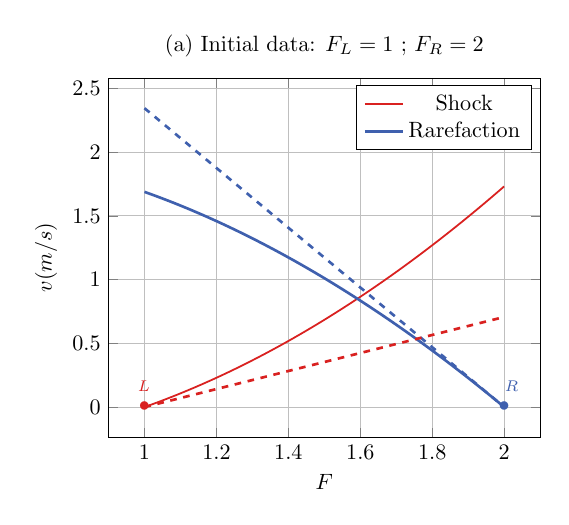
\begin{tikzpicture}[scale=0.8]
\begin{axis}[xlabel=$F$,ylabel=$v (m/s)$,ymajorgrids=true,xmajorgrids=true, title={(a) Initial data: $F_L=1$ ; $F_R=2$}]
  \addplot[Red,thick] coordinates {(1.0,0.0) (1.0196019601960196,0.019889905868838792) (1.0392039203920391,0.04035480171519238) (1.058805880588059,0.06139339246981025) (1.0784078407840785,0.08300445472552491) (1.098009800980098,0.1051868317293367) (1.1176117611761176,0.1279394287977403) (1.1372137213721372,0.1512612091133456) (1.1568156815681567,0.17515118986560513) (1.1764176417641765,0.19960843870261852) (1.196019601960196,0.2246320704646163) (1.2156215621562156,0.25022124417291264) (1.2352235223522352,0.2763751602509047) (1.2548254825482548,0.30309305795616337) (1.2744274427442743,0.330374213004825) (1.2940294029402941,0.3582179353714115) (1.3136313631363137,0.386623567248899) (1.3332333233323332,0.4155904811553686) (1.3528352835283528,0.445118078174895) (1.3724372437243724,0.47520578632153143) (1.3920392039203922,0.5058530590163028) (1.4116411641164117,0.5370593736680643) (1.4312431243124313,0.568824230349938) (1.4508450845084508,0.6011471505637854) (1.4704470447044704,0.6340276760858663) (1.4900490049004902,0.667465367887438) (1.5096509650965095,0.7014598051246006) (1.5292529252925293,0.7360105841921958) (1.5488548854885489,0.7711173178369951) (1.5684568456845684,0.8067796343258441) (1.5880588058805882,0.8429971766647708) (1.6076607660766076,0.8797696018654025) (1.6272627262726274,0.917096580255355) (1.646864686468647,0.9549777948294852) (1.6664666466646665,0.9934129406392047) (1.686068606860686,1.032401724217221) (1.7056705670567056,1.0719438630353144) (1.7252725272527254,1.1120390849929296) (1.7448744874487447,1.1526871279345328) (1.7644764476447645,1.1938877391938512) (1.784078407840784,1.2356406751632294) (1.8036803680368036,1.2779457008865038) (1.8232823282328234,1.320802589673878) (1.8428842884288428,1.3642111227374165) (1.8624862486248626,1.4081710888458763) (1.8820882088208821,1.4526822839976499) (1.9016901690169017,1.4977445111107466) (1.9212921292129215,1.543357579728744) (1.9408940894089408,1.5895213057417645) (1.9604960496049606,1.6362355111215798) (1.9800980098009802,1.6835000236699957) (1.9996999699969997,1.7313146767797576) };
  \addplot[Blue,very thick] coordinates {(1.0,1.6884673989302577) (1.0196019601960196,1.6685781823289632) (1.0392039203920391,1.648117983645035) (1.058805880588059,1.6270917763366024) (1.0784078407840785,1.6055041425368688) (1.098009800980098,1.5833593157699348) (1.1176117611761176,1.5606612177002648) (1.1372137213721372,1.5374134899261505) (1.1568156815681567,1.5136195216278194) (1.1764176417641765,1.48928247372591) (1.196019601960196,1.4644053000848238) (1.2156215621562156,1.4389907661996928) (1.2352235223522352,1.4130414657294894) (1.2548254825482548,1.3865598351776642) (1.2744274427442743,1.3595481669723095) (1.2940294029402941,1.3320086211576845) (1.3136313631363137,1.3039432358761032) (1.3332333233323332,1.2753539367920979) (1.3528352835283528,1.246242545588463) (1.3724372437243724,1.216610787645106) (1.3920392039203922,1.1864602989961286) (1.4116411641164117,1.1557926326474621) (1.4312431243124313,1.12460926432638) (1.4508450845084508,1.092911597724879) (1.4704470447044704,1.0607009692909792) (1.4900490049004902,1.0279786526152188) (1.5096509650965095,0.994745862453826) (1.5292529252925293,0.9610037584250569) (1.5488548854885489,0.9267534484108921) (1.5684568456845684,0.8919959916925568) (1.5880588058805882,0.8567324018451127) (1.6076607660766076,0.8209636494135533) (1.6272627262726274,0.7846906643903794) (1.646864686468647,0.7479143385125069) (1.6664666466646665,0.7106355273934435) (1.686068606860686,0.6728550525050632) (1.7056705670567056,0.6345737030218022) (1.7252725272527254,0.595792237538853) (1.7448744874487447,0.5565113856747698) (1.7644764476447645,0.5167318495678894) (1.784078407840784,0.47645430527509447) (1.8036803680368036,0.43567940408061234) (1.8232823282328234,0.3944077737218566) (1.8428842884288428,0.3526400195386741) (1.8624862486248626,0.31037672555176576) (1.8820882088208821,0.2676184554755838) (1.9016901690169017,0.22436575367049583) (1.9212921292129215,0.18061914603862234) (1.9408940894089408,0.13637914086738703) (1.9604960496049606,0.09164622962443836) (1.9800980098009802,0.04642088770736517) (1.9996999699969997,0.0007035751512764867) };
  \node at (axis cs:1,0) [Red] {$\bullet$};
  \node at (axis cs:2.,0) [Blue] {$\bullet$};
  \node at (axis cs:1,0) [anchor=south,Red] {$\Qcb^L$};
  \node at (axis cs:1.98,0) [above right,Blue] {$\Qcb^R$};
  \addplot[Blue,dashed,very thick,domain=1:2,samples=51,samples y=0]
    ({x},{0.-sqrt(0.5*(12.-1))*(x-2.)});
  \addplot[Red,dashed,very thick,domain=1:2,samples=51,samples y=0]
    ({x},{0.+sqrt(0.5*(2.-1))*(x-1.)});
  \legend{Shock,Rarefaction}
\end{axis}
\end{tikzpicture}
 \phantomsubcaption \label{subfig:SVK_Approx1}}
  % {\definecolor{Purple}{RGB}{120,28,129}
\definecolor{Blue}{RGB}{63,96,174}
\definecolor{Duck}{RGB}{83,158,182}
\definecolor{Green}{RGB}{109,179,136}
\definecolor{Yellow}{RGB}{202,184,67}
\definecolor{Orange}{RGB}{231,133,50}
\definecolor{Red}{RGB}{217,33,32}
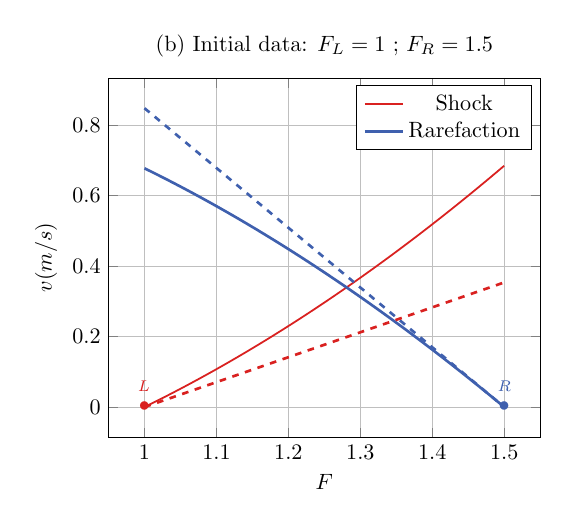
\begin{tikzpicture}[scale=0.8]
\begin{axis}[xlabel=$F$,ylabel=$v (m/s)$,ymajorgrids=true,xmajorgrids=true,title={(b) Initial data: $F_L=1$ ; $F_R=1.5$}]
\addplot[Red,thick] coordinates {(1.0,0.0) (1.00980098009801,0.009872995299740863) (1.0196019601960196,0.019889905868838792) (1.0294029402940295,0.030050562728014697) (1.0392039203920391,0.04035480171519238) (1.049004900490049,0.050802463310633685) (1.058805880588059,0.06139339246981025) (1.0686068606860686,0.07212743846361445) (1.0784078407840785,0.08300445472552491) (1.0882088208820881,0.09402429870536679) (1.098009800980098,0.1051868317293367) (1.1078107810781077,0.11649191886596709) (1.1176117611761176,0.1279394287977403) (1.1274127412741275,0.13952923369806353) (1.1372137213721372,0.1512612091133456) (1.147014701470147,0.16313523384992432) (1.1568156815681567,0.17515118986560513) (1.1666166616661666,0.18730896216559562) (1.1764176417641765,0.19960843870261852) (1.1862186218621862,0.21204951028101032) (1.196019601960196,0.2246320704646163) (1.2058205820582057,0.23735601548830068) (1.2156215621562156,0.25022124417291264) (1.2254225422542255,0.2632276578435396) (1.2352235223522352,0.2763751602509047) (1.245024502450245,0.2896636574957637) (1.2548254825482548,0.30309305795616337) (1.2646264626462647,0.31666327221743923) (1.2744274427442743,0.330374213004825) (1.2842284228422842,0.3442257951185647) (1.2940294029402941,0.3582179353714115) (1.3038303830383038,0.3723505525284153) (1.3136313631363137,0.386623567248899) (1.3234323432343236,0.40103690203052456) (1.3332333233323332,0.4155904811553686) (1.343034303430343,0.43028423063791627) (1.3528352835283528,0.445118078174895) (1.3626362636263627,0.46009195309686984) (1.3724372437243724,0.47520578632153143) (1.3822382238223823,0.49045951030860363) (1.3920392039203922,0.5058530590163028) (1.4018401840184018,0.5213863678592919) (1.4116411641164117,0.5370593736680643) (1.4214421442144214,0.5528720146496987) (1.4312431243124313,0.568824230349938) (1.441044104410441,0.584915961616529) (1.4508450845084508,0.6011471505637854) (1.4606460646064607,0.6175177405383133) (1.4704470447044704,0.6340276760858663) (1.4802480248024803,0.6506769029192789) (1.4900490049004902,0.667465367887438) (1.4998499849984999,0.6843930189452551) };
\addplot[Blue,very thick] coordinates {(1.0,0.6772957538163167) (1.00980098009801,0.6674228457131514) (1.0196019601960196,0.6574065372150225) (1.0294029402940295,0.6472474900740499) (1.0392039203920391,0.636946338531094) (1.049004900490049,0.6265036909324323) (1.058805880588059,0.6159201312226612) (1.0686068606860686,0.6051962203255077) (1.0784078407840785,0.594332497422928) (1.0882088208820881,0.5833294811417358) (1.098009800980098,0.5721876706559943) (1.1078107810781077,0.5609075467125532) (1.1176117611761176,0.5494895725863237) (1.1274127412741275,0.5379341949712366) (1.1372137213721372,0.5262418448122094) (1.147014701470147,0.5144129380829412) (1.1568156815681567,0.5024478765138787) (1.1666166616661666,0.4903470482742829) (1.1764176417641765,0.47811082861196913) (1.1862186218621862,0.46573958045394287) (1.196019601960196,0.45323365497088286) (1.2058205820582057,0.4405933921081488) (1.2156215621562156,0.427819121085752) (1.2254225422542255,0.4149111608695282) (1.2352235223522352,0.40186982061554877) (1.245024502450245,0.38869540008963877) (1.2548254825482548,0.3753881900637237) (1.2646264626462647,0.36194847269056873) (1.2744274427442743,0.3483765218583685) (1.2842284228422842,0.3346726035265095) (1.2940294029402941,0.320836976043744) (1.3038303830383038,0.30686989044989726) (1.3136313631363137,0.2927715907621622) (1.3234323432343236,0.2785423142469442) (1.3332333233323332,0.26418229167815693) (1.343034303430343,0.2496917475827887) (1.3528352835283528,0.23507090047452192) (1.3626362636263627,0.2203199630761068) (1.3724372437243724,0.205439142531165) (1.3822382238223823,0.190428640606026) (1.3920392039203922,0.1752886538821878) (1.4018401840184018,0.1600193739399201) (1.4116411641164117,0.14462098753352123) (1.4214421442144214,0.12909367675868896) (1.4312431243124313,0.11343761921243899) (1.441044104410441,0.09765298814598275) (1.4508450845084508,0.08173995261093799) (1.4606460646064607,0.0656986775992334) (1.4704470447044704,0.04952932417703831) (1.4802480248024803,0.03323204961302656) (1.4900490049004902,0.016807007501277855) (1.4998499849984999,0.000254347879077443) };
\node at (axis cs:1,0) [Red] {$\bullet$};
  \node at (axis cs:1.5,0) [Blue] {$\bullet$};
  \node at (axis cs:1,0) [anchor=south,Red] {$\Qcb^L$};
  \node at (axis cs:1.48,0) [above right,Blue] {$\Qcb^R$};
  \addplot[Blue,dashed,very thick,domain=1:1.5,samples=51,samples y=0]
    ({x},{0.-sqrt(0.5*(3.*(1.5^2)-1))*(x-1.5)});
  \addplot[Red,dashed,very thick,domain=1:1.5,samples=51,samples y=0]
  ({x},{0.+sqrt(0.5*(2.-1))*(x-1.)});
  \legend{Shock,Rarefaction}
\end{axis}
\end{tikzpicture}
 \phantomsubcaption \label{subfig:SVK_Approx2}} \\
  % {\definecolor{Red}{RGB}{217,33,32}
\definecolor{Blue}{RGB}{63,96,174}
\definecolor{Duck}{RGB}{83,158,182}
\definecolor{Green}{RGB}{109,179,136}
\definecolor{Yellow}{RGB}{202,184,67}
\definecolor{Orange}{RGB}{231,133,50}
\definecolor{Purple}{RGB}{120,28,129}
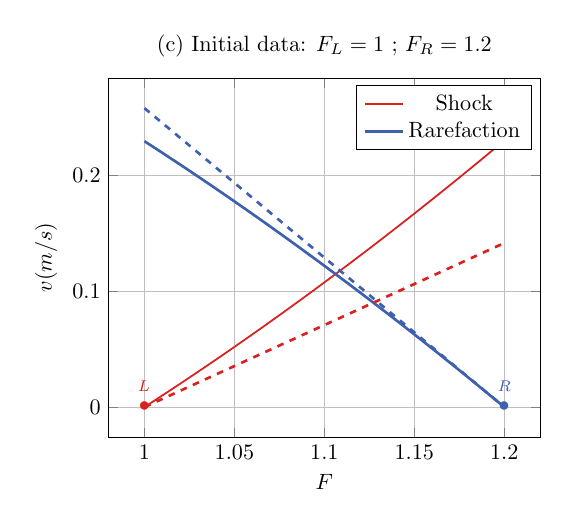
\begin{tikzpicture}[scale=0.8]
\begin{axis}[xlabel=$F$,ylabel=$v (m/s)$,ymajorgrids=true,xmajorgrids=true,title={(c) Initial data: $F_L=1$ ; $F_R=1.2$}]
\addplot[Red,thick] coordinates {(1.0,0.0) (1.003920392039204,0.003931917267080632) (1.0078407840784078,0.007886877524091035) (1.0117611761176117,0.011864869670167599) (1.0156815681568157,0.01586588273338493) (1.0196019601960196,0.019889905868838792) (1.0235223522352235,0.023936928356764118) (1.0274427442744274,0.028006939600686957) (1.0313631363136313,0.03209992912561001) (1.0352835283528352,0.0362158865762309) (1.0392039203920391,0.04035480171519238) (1.043124312431243,0.04451666442136419) (1.047044704470447,0.04870146468815503) (1.0509650965096509,0.0529091926218551) (1.0548854885488548,0.05713983844000771) (1.0588058805880587,0.06139339246981002) (1.0627262726272626,0.06566984514654124) (1.0666466646664667,0.06996918701201955) (1.0705670567056704,0.07429140871308397) (1.0744874487448746,0.07863650100010654) (1.0784078407840785,0.08300445472552491) (1.0823282328232824,0.08739526084240548) (1.0862486248624863,0.09180891040302837) (1.0901690169016902,0.09624539455749745) (1.0940894089408941,0.1007047045523746) (1.098009800980098,0.1051868317293367) (1.101930193019302,0.10969176752385594) (1.1058505850585059,0.11421950346390249) (1.1097709770977098,0.11877003116866883) (1.1136913691369137,0.12334334234731587) (1.1176117611761176,0.1279394287977403) (1.1215321532153215,0.13255828240536205) (1.1254525452545254,0.1371998951419326) (1.1293729372937293,0.14186425906436276) (1.1332933293329333,0.14655136631357016) (1.1372137213721372,0.1512612091133456) (1.141134113411341,0.15599377976923837) (1.145054505450545,0.16074907066745941) (1.148974897489749,0.1655270742738032) (1.1528952895289528,0.17032778313258656) (1.1568156815681567,0.17515118986560513) (1.1607360736073606,0.17999728717110672) (1.1646564656465646,0.18486606782278137) (1.1685768576857685,0.18975752466876733) (1.1724972497249724,0.19467165063067376) (1.1764176417641763,0.19960843870261824) (1.1803380338033802,0.20456788195028056) (1.1842584258425841,0.20954997350997065) (1.188178817881788,0.21455470658771253) (1.192099209920992,0.21958207445834133) (1.196019601960196,0.2246320704646163) (1.1999399939993998,0.229704688016345) };
\addplot[Blue,very thick] coordinates {(1.0,0.22917941198468886) (1.003920392039204,0.2252475003389243) (1.0078407840784078,0.22129257921328083) (1.0117611761176117,0.21731469262755104) (1.0156815681568157,0.21331388384346875) (1.0196019601960196,0.20929019538339458) (1.0235223522352235,0.20524366904839547) (1.0274427442744274,0.20117434593574032) (1.0313631363136313,0.19708226645583485) (1.0352835283528352,0.19296747034862255) (1.0392039203920391,0.18882999669946615) (1.043124312431243,0.184669883954535) (1.047044704470447,0.1804871699357172) (1.0509650965096509,0.1762818918550712) (1.0548854885488548,0.17205408632883865) (1.0588058805880587,0.1678037893910336) (1.0627262726272626,0.16353103650662262) (1.0666466646664667,0.15923586258431413) (1.0705670567056704,0.1549183019889692) (1.0744874487448746,0.15057838855364641) (1.0784078407840785,0.1462161555913001) (1.0823282328232824,0.14183163590613646) (1.0862486248624863,0.13742486180464666) (1.0901690169016902,0.1329958651063243) (1.0940894089408941,0.12854467715408055) (1.098009800980098,0.12407132882436642) (1.101930193019302,0.11957585053701415) (1.1058505850585059,0.11505827226480363) (1.1097709770977098,0.11051862354276928) (1.1136913691369137,0.10595693347725012) (1.1176117611761176,0.10137323075469579) (1.1215321532153215,0.09676754365023553) (1.1254525452545254,0.09213990003601796) (1.1293729372937293,0.08749032738932871) (1.1332933293329333,0.08281885280049482) (1.1372137213721372,0.07812550298058156) (1.141134113411341,0.07341030426888846) (1.145054505450545,0.0686732826402522) (1.148974897489749,0.06391446371216106) (1.1528952895289528,0.05913387275168875) (1.1568156815681567,0.05433153468225065) (1.1607360736073606,0.04950747409019151) (1.1646564656465646,0.04466171523120707) (1.1685768576857685,0.03979428203660571) (1.1724972497249724,0.03490519811941557) (1.1764176417641763,0.029994486780341414) (1.1803380338033802,0.025062171013576353) (1.1842584258425841,0.020108273512470697) (1.188178817881788,0.015132816675066284) (1.192099209920992,0.010135822609495795) (1.196019601960196,0.0051173131392549635) (1.1999399939993998,7.730980834955399e-05) };
\legend{Shock,Rarefaction}
\node at (axis cs:1,0) [Red] {$\bullet$};
  \node at (axis cs:1.2,0) [Blue] {$\bullet$};
  \node at (axis cs:1,0) [anchor=south,Red] {$\Qcb^L$};
  \node at (axis cs:1.192,0) [above right,Blue] {$\Qcb^R$};
  \addplot[Blue,dashed,very thick,domain=1:1.2,samples=51,samples y=0]
    ({x},{0.-sqrt(0.5*(3.*(1.2^2)-1))*(x-1.2)});
  \addplot[Red,dashed,very thick,domain=1:1.2,samples=51,samples y=0]
  ({x},{0.+sqrt(0.5*(2.-1))*(x-1.)});
\legend{Shock,Rarefaction}
\end{axis}
\end{tikzpicture}
 \phantomsubcaption \label{subfig:SVK_Approx3}}
  {\definecolor{Red}{RGB}{217,33,32}
\definecolor{Blue}{RGB}{63,96,174}
\definecolor{Duck}{RGB}{83,158,182}
\definecolor{Green}{RGB}{109,179,136}
\definecolor{Yellow}{RGB}{202,184,67}
\definecolor{Orange}{RGB}{231,133,50}
\definecolor{Purple}{RGB}{120,28,129}
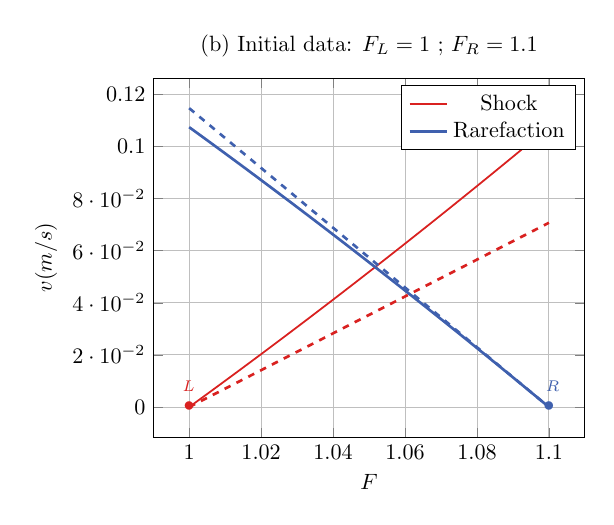
\begin{tikzpicture}[scale=0.8]
\begin{axis}[xlabel=$F$,ylabel=$v (m/s)$,ymajorgrids=true,xmajorgrids=true,title={(b) Initial data: $F_L=1$ ; $F_R=1.1$}]
\addplot[Red,thick] coordinates {(1.0,0.0) (1.001960196019602,0.0019630775609053948) (1.003920392039204,0.003931917267080632) (1.005880588058806,0.005906517718693416) (1.0078407840784078,0.007886877524091035) (1.00980098009801,0.009872995299740863) (1.0117611761176117,0.011864869670167599) (1.0137213721372138,0.01386249926789511) (1.0156815681568157,0.01586588273338493) (1.0176417641764177,0.01787501871497885) (1.0196019601960196,0.019889905868838792) (1.0215621562156216,0.02191054285889049) (1.0235223522352235,0.023936928356764118) (1.0254825482548255,0.025969061041739377) (1.0274427442744274,0.028006939600686957) (1.0294029402940295,0.030050562728014697) (1.0313631363136313,0.03209992912561001) (1.0333233323332334,0.034155037502787186) (1.0352835283528352,0.0362158865762309) (1.0372437243724373,0.03828247506994398) (1.0392039203920391,0.04035480171519238) (1.0411641164116412,0.04243286525045405) (1.0431243124312433,0.044516664421364406) (1.045084508450845,0.04660619798066565) (1.0470447044704472,0.048701464688155255) (1.049004900490049,0.050802463310633685) (1.050965096509651,0.05290919262185532) (1.052925292529253,0.055021651402476585) (1.054885488548855,0.05713983844000798) (1.0568456845684568,0.059263752528762766) (1.058805880588059,0.06139339246981025) (1.0607660766076608,0.06352875707092508) (1.0627262726272628,0.06566984514654145) (1.0646864686468647,0.06781665551770343) (1.0666466646664667,0.06996918701201955) (1.0686068606860686,0.07212743846361445) (1.0705670567056706,0.07429140871308419) (1.0725272527252725,0.07646109660744838) (1.0744874487448746,0.07863650100010654) (1.0764476447644764,0.08081762075079126) (1.0784078407840785,0.08300445472552491) (1.0803680368036805,0.08519700179657394) (1.0823282328232824,0.08739526084240548) (1.0842884288428845,0.08959923074764438) (1.0862486248624863,0.09180891040302837) (1.0882088208820884,0.09402429870536706) (1.0901690169016902,0.09624539455749745) (1.0921292129212923,0.09847219686824406) (1.0940894089408941,0.1007047045523746) (1.0960496049604962,0.10294291653056116) (1.098009800980098,0.1051868317293367) (1.0999699969997,0.10743644908105657) };
\addplot[Blue,very thick] coordinates {(1.0,0.1073874627707086) (1.001960196019602,0.10542438591418365) (1.003920392039204,0.10345555112494406) (1.005880588058806,0.10148096397787983) (1.0078407840784078,0.09950062999930058) (1.00980098009801,0.09751455466754301) (1.0117611761176117,0.09552274341357074) (1.0137213721372138,0.09352520162156171) (1.0156815681568157,0.0915219346294884) (1.0176417641764177,0.089512947729686) (1.0196019601960196,0.08749824616941433) (1.0215621562156216,0.08547783515140679) (1.0235223522352235,0.08345171983441528) (1.0254825482548255,0.08141990533374051) (1.0274427442744274,0.07938239672176006) (1.0294029402940295,0.07733919902844166) (1.0313631363136313,0.0752903172418546) (1.0333233323332334,0.07323575630866758) (1.0352835283528352,0.07117552113464229) (1.0372437243724373,0.06910961658511733) (1.0392039203920391,0.06703804748548585) (1.0411641164116412,0.06496081862166392) (1.0431243124312433,0.06287793474055453) (1.045084508450845,0.06078940055050131) (1.0470447044704472,0.05869522072173673) (1.049004900490049,0.056595399886824015) (1.050965096509651,0.05448994264109064) (1.052925292529253,0.05237885354305752) (1.054885488548855,0.05026213711485809) (1.0568456845684568,0.0481397978426566) (1.058805880588059,0.04601184017705303) (1.0607660766076608,0.04387826853348905) (1.0627262726272628,0.0417390872926421) (1.0646864686468647,0.0395943008008181) (1.0666466646664667,0.037443913370333926) (1.0686068606860686,0.03528792927989956) (1.0705670567056706,0.03312635277498877) (1.0725272527252725,0.03095918806820985) (1.0744874487448746,0.02878643933966615) (1.0764476447644764,0.026608110737315303) (1.0784078407840785,0.0244242063773199) (1.0803680368036805,0.022234730344396287) (1.0823282328232824,0.020039686692156212) (1.0842884288428845,0.017839079443443134) (1.0862486248624863,0.01563291259066641) (1.0882088208820884,0.013421190096127349) (1.0901690169016902,0.011203915892344065) (1.0921292129212923,0.008981093882367926) (1.0940894089408941,0.006752727940100287) (1.0960496049604962,0.00451882191059879) (1.098009800980098,0.0022793796103861676) (1.0999699969997,3.4404827748516585e-05) };
\node at (axis cs:1,0) [Red] {$\bullet$};
  \node at (axis cs:1.1,0) [Blue] {$\bullet$};
  \node at (axis cs:1,0) [anchor=south,Red] {$\Qcb^L$};
  \node at (axis cs:1.097,0) [above right,Blue] {$\Qcb^R$};
  \addplot[Red,dashed,very thick,domain=1:1.1,samples=51,samples y=0]
  ({x},{0.+sqrt(0.5*(2.-1))*(x-1.)});
  \addplot[Blue,dashed,very thick,domain=1:1.1,samples=51,samples y=0]
    ({x},{0.-sqrt(0.5*(3.*(1.1^2)-1))*(x-1.1)});
\legend{Shock,Rarefaction}
\end{axis}
\end{tikzpicture}
 \phantomsubcaption \label{subfig:SVK_Approx4}}
  \caption{Comparison of approximate (dashed curves) and exact (solid curves) solution for a one-dimensional strain problem in a Saint-Venant-Kirchhoff hyperelastic material}
  \label{fig:comparison_exact_approx}
\end{figure}

Figure \ref{fig:comparison_exact_approx} shows comparisons of approximate and exact solutions for various initial data, all leading to a $1$-shock, $2$-rarefaction solution. As expected, approximate and exact solutions are very different for high loads (figures \ref{fig:comparison_exact_approx}\subref{subfig:SVK_Approx1}) and get closer for initial discontinuities falling the linearization assumption $\Qcb^L\approx \Qcb^R$ (figures \ref{fig:comparison_exact_approx}\subref{subfig:SVK_Approx4}).
\subsection{Elastoplastic solids}
Linear hardening
Not an approximate solver but an exact one with prediction correction steps.
The solution of such problems may involve up to two sets of waves, each of which corresponding to either elastic or plastic discontinuous waves. Indeed, the tangent modulus being discontinuous through the plastic threshold, the characteristic analysis of the Jacobian matrix leads in this case to two eigenvalues $\pm c$ for elastic evolutions, and two eigenvalues $\pm c_p$ for plastic ones. Figure \ref{fig:EP_bar_solution}\subref{subfig:ep_bar_charac} shows the characteristic structure of the solution in the case of initial data leading to plastic flow in both sides of the initial discontinuity the Riemann data. However, whether a plastic wave must be added or not to elastic ones depends on the projection of the stress propagated by elastic discontinuities. Hence, the approximate Riemann solver requires in the case of elastoplasticity prediction and correction steps where the trial state is computed as a purely elastic one with equation \eqref{eq:solution_charac_variables}. Then, testing the trial test against the yield criterion on both sides allows to determine whether plastic flow occurs, in which case a plastic wave must be added. The yield function remaining null 

Approximate solver that can be seen as a prediction-correction procedure developed in \cite{Fogarty} based on the analytical solution \cite{Wang}.

The problem considered now involve an elastoplastic infinite one-dimensional medium with linear hardening in which initial data are given so that $v(x>0,0)=-v(x<0,0),\bar{v}$ while stress and plastic strain components are considered to be zero everywhere. The prescribed velocity is defined as:
\begin{equation}
  \label{eq:Hugoniot_velocity}
  \bar{v}>\frac{\lambda+2\mu}{2\mu \rho c}\sigma_y
\end{equation}
Analytical solution \cite{Thomas_EP}, linear hardening, initially undeformed $\eps^p=0 \forall x$, elastic limit, tangent modulus \cite{Simo}, von mises :
\begin{figure}[h!]
  \centering
  \subcaptionbox{Characteristic structure of the solution of the elastoplastic Riemann problem\label{subfig:ep_bar_charac}}{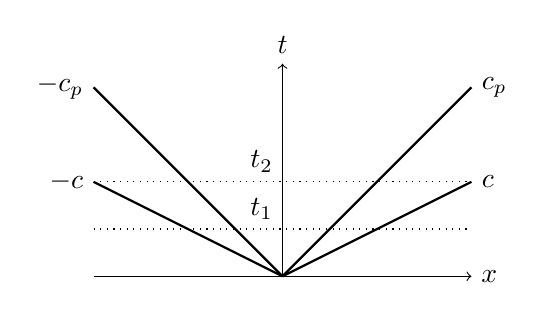
\begin{tikzpicture}[scale=0.6]
  \draw[->] (-4,0) -- (4.,0) node[right] {$x$};
  \draw[->] (0,0) -- (0,4.5) node[above] {$t$};
  \draw[thick] (0,0) -- (4.,2) node [right] {$c$};
  \draw[thick] (0,0) -- (4.,4) node [right] {$c_p$};
  \draw[thick] (0,0) -- (-4.,2) node [left] {$-c$};
  \draw[thick] (0,0) -- (-4.,4) node [left] {$-c_p$};
  \draw[dotted] (-4,1.)-- (0,1) node [above left] {$t_1$} --(4.,1);
  \draw[dotted] (-4,2.)-- (0,2) node [above left] {$t_2$} --(4.,2);
\end{tikzpicture}

%%% Local Variables:
%%% mode: latex
%%% TeX-master: "../../mainManuscript"
%%% End:}
  \subcaptionbox{Stress profiles in the bar \label{subfig:ep_bar_stress}}{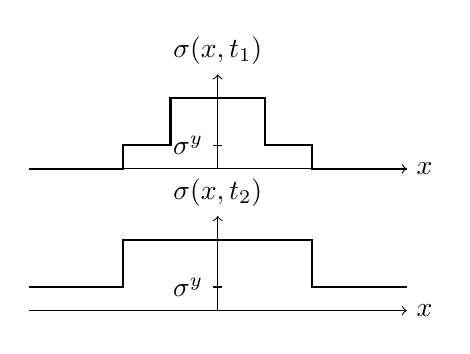
\begin{tikzpicture}[scale=0.6]
\draw[->] (0,0) -- (0,2) node [above] {$\sigma(x,t_1)$};
\draw[->] (-4,0) -- (4,0) node [right] {$x$};
\draw[thick] (-4,0) --(-2,0) -- (-2,0.5) -- (-1,0.5) -- (-1,1.5) -- (1,1.5) -- (1,0.5) -- (2,0.5) -- (2,0) -- (4,.0);
\draw (-0.1,0.5) node[left] {$\sigma^y$}-- (0.1,0.5);

\draw[->] (0,0-3) -- (0,2-3) node [above] {$\sigma(x,t_2)$};
\draw[->] (-4,0-3) -- (4,0-3) node [right] {$x$};
\draw[thick] (-4,0.5-3)  -- (-2,0.5-3)  --(-2,1.5-3) -- (2,1.5-3) -- (2,.5-3) -- (4,.5-3);
\draw (-0.1,0.5-3) node[left] {$\sigma^y$}-- (0.1,0.5-3);

\end{tikzpicture}}
  \caption{Solution of Riemann problem in elastoplastic bars (linear hardening)}
  \label{fig:EP_bar_solution}
\end{figure}
$\Qcb=\matrice{v \\ \sigma} ;\Fcb=\matrice{-\frac{1}{\rho}\sigma \\ -H v} ; \Jbsf=-\matrice{0 & \frac{1}{\rho}\\ H& 0 } $ where H is the tangent modulus $\lambda+2\mu ; \beta$
% \subsection{Elastic and elastic-viscoplastic solids}
% \subsubsection{Linear elastic plane bar}
% \subsubsection{Linear elastic plane wave}
% \subsubsection{Elastoviscoplasic bar and plane wave}
% %\subsubsection{Elastoviscoplasic}
% \subsection{Elastoplastic solids}
% \subsubsection{Linearly hardening media}
% \subsubsection{Decreasingly hardening media}
% \subsection{Saint-Venant-Kirchhoff hyperelastic solids}

%%% Local Variables:
%%% mode: latex
%%% TeX-master: "../mainManuscript"
%%% End:
